\documentclass{article} % For LaTeX2e
\usepackage{nips15submit_e,times}
\usepackage{hyperref}
\usepackage{url}
\usepackage{graphicx}
\usepackage{multirow}
%\documentstyle[nips14submit_09,times,art10]{article} % For LaTeX 2.09


\title{CSC 522 - Comparison of Encoding and Classification Methodologies for Prediction of Grant Applications}


\author{
	Priyaranjan Behera\\
	Department of Computer Science\\
	North Carolina State University\\
	\texttt{pbehera@ncsu.edu} \\
	\And
	Sai Sri Harsha Kunapareddy\\
	Department of Computer Science\\
	North Carolina State University\\
	\texttt{skunapa@ncsu.edu} \\
}

% The \author macro works with any number of authors. There are two commands
% used to separate the names and addresses of multiple authors: \And and \AND.
%
% Using \And between authors leaves it to \LaTeX{} to determine where to break
% the lines. Using \AND forces a linebreak at that point. So, if \LaTeX{}
% puts 3 of 4 authors names on the first line, and the last on the second
% line, try using \AND instead of \And before the third author name.

\newcommand{\fix}{\marginpar{FIX}}
\newcommand{\new}{\marginpar{NEW}}

\nipsfinalcopy % Uncomment for camera-ready version

\begin{document}
	
	
	\maketitle
	
	\section{Background}
	
	Around the world, the pool of funds available for research grants is steadily shrinking (in a relative sense). In Australia, success rates have fallen to 20-25 per cent, meaning that most academics are spending valuable time making applications that end up being rejected. This problem was hosted as a competition by University of Melbourne to address their inefficiencies with the grant applications. There is also a hope of discovering the most important criteria that are required to succeed in a grant application. 
	
	\subsection{Problem}
	
	The university has provided a dataset containing 249 features, including variables that represent:
	
	\begin{itemize}
		\item Type and size of the grant: It includes the basic information of the Grant Application like Application Month, Year, Contract Value, Sponsors, etc.
		\item General area of study in the grant application: It includes the information on the study that is intended to be done with the grant like  research fields, courses and disciplines class and socio economic objective class.
		\item De-identified Information of the Investigators: It includes personal data of the investigators like number of publications in different levels of journals, past history in grant applications, experience, educational qualifications, etc.  
	\end{itemize}
	
	The dataset contains multi-variate data with a few of them being continuous variables and a few categorical. There is a variable number of investigators in an application and thus, we need to aggregate the person data to create an efficient model. We implemented several of the classification techniques covered in the CSC522 course to arrive upon an efficient model.
	
	
	\subsection{Literature Survey}
	
	As the dataset contains a variable number of person attributes depending on the number of investigators in a grant application, it would lead to multiple missing data fields in applications where the investigator count is less. According to Gerhard Svolba \cite{OneRow}, we need to create a one-row-per-subject data mart for most of the analytical methods that we need to proceed with. Accordingly, we need to aggregate the person data using mean, median, standard deviation, the quartiles, or special quantiles, etc to create the input rows.
	
	We looked at approaches taken to solve similar problems which contains both continuous and categorical data \cite{Matlab} and found that decision trees and Naive Bayes are popular choices. On the contrary, methods like neural networks, SVM, etc. cannot work with categorical data. We implement decision trees as well as bagged and boosted trees for more efficiency. 
	
	Daniele et al. \cite{HighCard} focused on the transformation of categorical data to continuous/binary data so that we can use the analytical methods which cannot process categorical data. While traditionally binary encoding is used for conversion of categorical data to binary, for categories with high cardinality a probabilistic approach is suggested.
	
	\section{Methods}
	
	The analysis of the data required extensive preprocessing steps because of its multi-variate nature and variable number of attributes. We implemented different type of classification techniques to compare the models and find the determining attributes for the classification.
	
	\subsection{Preprocessing}
	
	To handle the categorical values in the data, we indexed the attributes with numerical values after finding the unique values for each of the attributes. As per the approach suggested by Gerhard Svolba \cite{OneRow}, we aggregated the variable number of investigators specific data for each of the application which is not null and found the minimum, maximum for all the attributes. While for continuous attributes we also calculated mean, median, sum of the values to create new features. We then created plots of the attributes with respect to the output to visually inspect any correlation of the attributes with the results.
	
	Since classification techniques like SVMs, Neural Networks, cannot handle categorical data, we implemented binary encoding to convert the categorical data into binary attributes which can be used in the analytical techniques. Further, to handle high cardinality, we implemented a probabilistic feature creation as specified at \cite{HighCard}. 
	
	\subsection{Classification}
	
	We implemented most of the classification techniques covered in CSC522 and compared their efficiencies.
	
	\subsubsection{Decision Tree and Random Forest}
	According to our survey of approaches employed for similar problems, decision tree turns out to be a popular choice. This attributes to the fact the it can handle categorical values without any further processing. We also implemented bagged trees using the dataset to get a more efficient classification. We also used the error rate obtained by changing values of attributes in a random forest to determine the most important factors which decide the success of a grant application.
	
	\subsubsection{Neural Networks}
	Since the neural networks can handle a high number of attributes, this will serve as an ideal classifier particularly when we use the binary encoding with a high cardinality of the categorical attributes. However, we cannot estimate the determining factors of an application though this method.
	
	\subsubsection{SVMs}
	SVM based classifers are known to work well with encoded data and thus, we executed the SVM based classifiers on the binary and probabilistic encoded data. We used the linear, quadratic and cubic kernels to find an effective model. 
	
	\section{Plan}
	According to the problem statement of the competition, we aimed to find a model which has a greater accuracy while minimizing the false positives in the output.
	
	\subsection{Hypothesis}
	We worked on implementing models of the classifications techniques we have been familiarized with to find a model with lesser number of false positives and higher accuracy. Thus, we focused on the values of True Positive Rate, False Negative Rate, Precision and Accuracy of the models. Most importantly, we used the ROC (Receiver Operating Curve) to determine the effectiveness of the model by comparing the area under the curve for the models. This will be more helpful compared to other criteria as:
	\begin{itemize}
		\item It is insensitive to unbalanced dataset where there is a disparity in the number of test cases outputs.  
		\item We consider all the cut-offs in a model to find its effectiveness.
	\end{itemize}
	
	We worked on experiments to test the technique of conversion of categorical attributes to probabilistic values for high cardinality attributes\cite{HighCard}. We considered the same evaluation parameters mentioned above to compare with models which use binary encoding. 
	
	We also worked on finding the most determining factors which decides the fate of an application. For this, we used the characteristic of the random forest libraries which find the effective factors in an input by measuring the error rate when an attribute value is changed. 
	\subsection{Experimental Design}
	\begin{enumerate}
		\item \emph{Data Indexing:} Since there are a large number of categorical attributes in the data, indexing was done to standardize them into integral values.
		\item \emph{Dimensionality Reduction and Data Creation:} Since the data has variable number of person data in each of the grant application, there was a need to aggregate the data to create similar rows for comparing applications. We used different aggregation functions like minimum, maximum, mean, median, sum of the attribute values for each of the person within a data row\cite{OneRow} to achieve this.
		\item \emph{Data Visualization:} Effectiveness of the attributes to determine the result of an application was studied by creating scatter plots and histograms for each of the attributes in the input matrix. 
		\item \emph{Handling of Categorical Attributes:} While techniques involving decision trees and naive bayes work well with categorical values, other methods need binary or continuous inputs. Thus, we will be adopting two methods to use the data in other classifiers:
		
		\begin{itemize}
			\item Binary encoding: In this technique, an indexed categorical variable with $N$ cardinality is converted to its binarized index value. 
			\item Probability Substitution: In this technique, the probability of getting the output as 1 is calculated for each of the values of the categorical variable. These values are used instead of the original variable values for the classifications.  \cite{HighCard}
		\end{itemize}  
		
		
		\item \emph{Classifications:} We used the different inputs obtained in the above steps to train and test the classifiers.
		\begin{itemize}
			\item Decision Tree
			\item Random Forest
			\item Boosted Trees
			\item Neural Networks
			\item SVMs
		\end{itemize}
		Primarily, libraries in Matlab will be used for this purpose where tools like 'classificationLearner', 'nntool' will be used in addition to other basic classifier classes.
		
		\item \emph{Factor Determination:} The random forest library explicitly determines the most important factor which decides the output. We will be using this to find out the factors which can improve the credentials of an application.
		
		\item \emph{Evaluation and Results:} Confusion matrices will be drawn for each of the classifications done in the experiments to find the accuracy, recall, precision and false positive rate. Additionally, ROC will be generated from the GUI interfaces in 'classificationLearner' and 'nntool'.
		
	\end{enumerate}
	
	
	\section{Experiments}
	
	After the pre-processing steps which included indexing and generation of new features, we resorted to visualization of the data to find any correlation of attributes with the results (As shown in Fig.\ref{fig:sponsor}).
	
	\begin{figure}[h]
		\begin{center}
			%\framebox[4.0in]{$\;$}
			\fbox{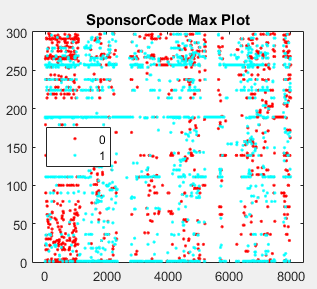
\includegraphics[scale=0.5]{SponsorPlot.png}}
			\fbox{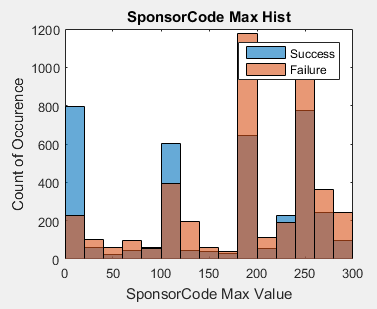
\includegraphics[scale=0.5]{SponsorHist.png}}
		\end{center}
		\caption{Scatter Plot and Histogram for Sponsor Codes.}
		\label{fig:sponsor}
	\end{figure}
	
	We take an example of one of the attributes, Sponsor code, for which we plot the data and see a discerning pattern. We can see that for specific sponsor codes, the chances of getting a grant is more.But we could not find any conclusive pattern in most of the plots and thus, moved on with the classification. 
	
	Since our data did not have too many attributes, dimensionality reduction was not required. For the decision tree and SVM classifiers we opted for a 5-fold cross validation. 
	
	After the classification models were implemented, we analyzed the confusion matrix to deduce the evaluation parameters and compare the models. One of the confusion matrices along with TPR/FNR rate which was obtained from the random forest model for categorical data is listed at Fig.\ref{fig:RFCM}. 
	
	\begin{figure}[h]
		\begin{center}
			%\framebox[4.0in]{$\;$}
			\fbox{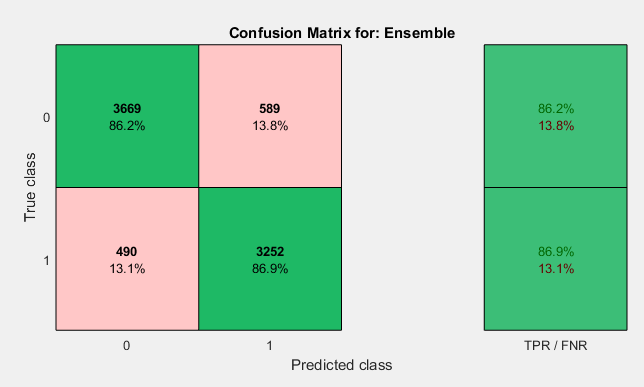
\includegraphics[scale=0.5]{RandomForestCM.png}}
		\end{center}
		\caption{Confusion Matrix and TPR/FNR of Random Forest on Categorical Data.}
		\label{fig:RFCM}
	\end{figure}
	
	

	
	We also compared the models according to the area under the curve of the ROC curve. This will help us to determine the effectiveness of the model in spite of any imbalance in the number of data objects with a specific output
	By comparing the models for categorical data with respect to the ROC curve(Fig.\ref{fig:ROCCat}), we find that the area under the curve for random forest is a little high and thus, random forest is a better model in this scenario where we take the data without any encoding.
	
	\begin{figure}[h]
		\begin{center}
			%\framebox[4.0in]{$\;$}
			\fbox{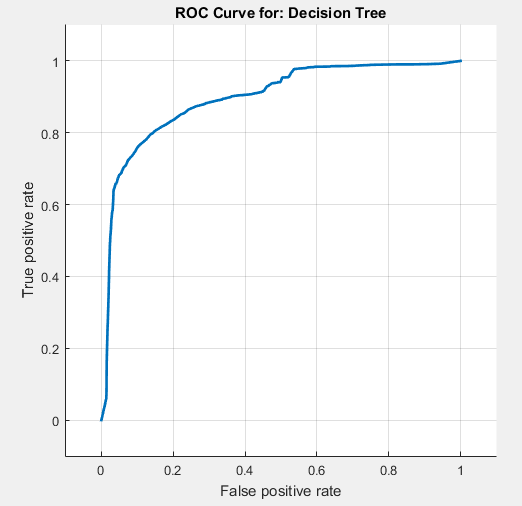
\includegraphics[scale=0.38]{ROC-DT.png}}
			\fbox{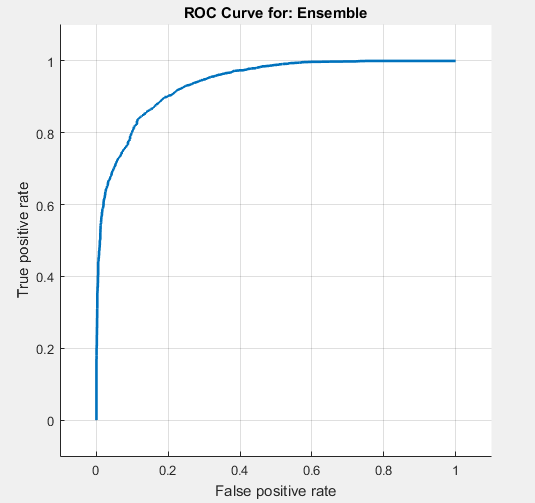
\includegraphics[scale=0.38]{ROC-RF.png}}
		\end{center}
		
		\caption{ROC Plot for Decision Tree and Random Forest.}
		\label{fig:ROCCat}
	\end{figure}
	
	Similarly, we can compare the encoding methodologies by using the same classification methodology for each of the encodings and evaluate the parameters. Fig. \ref{fig:ROC} provides the comparision between the encodings where we have taken quadratic SVM as the classifier. We see that binary encoding works a little better in this scenario.
	
	\begin{figure}[h]
		\begin{center}
			%\framebox[4.0in]{$\;$}
			\fbox{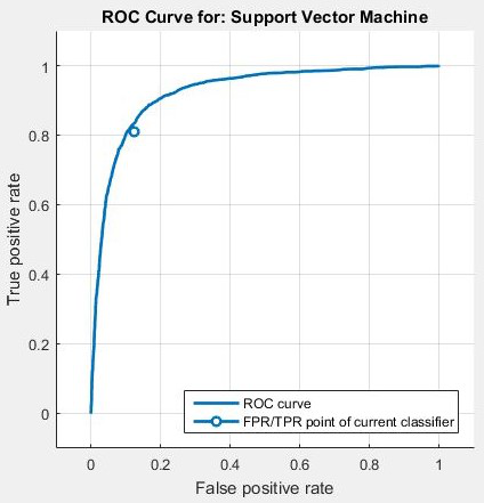
\includegraphics[scale=0.4]{ROC-QuadSVM-Bin.png}}
			\fbox{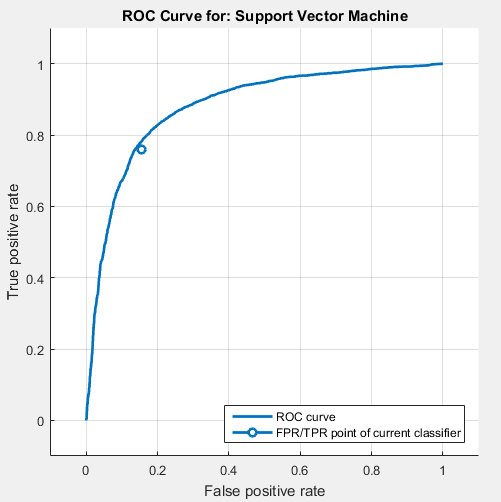
\includegraphics[scale=0.4]{ROC-QuadSVM-Prob.png}}
		\end{center}
		
		\caption{ROC Plot for Decision Tree and Random Forest.}
		\label{fig:ROCProbBin}
	\end{figure}
	
	In addition, we found the important features which determine the outcome of the application. The data is plotted in Fig.\ref{fig:FIM}. From the plot we can see that features Contract Value(3), Sponsor Code(1), Application Month(14), Grant Category(2) are the most important factors.
	
	\begin{figure}[h]
		\begin{center}
			%\framebox[4.0in]{$\;$}
			\fbox{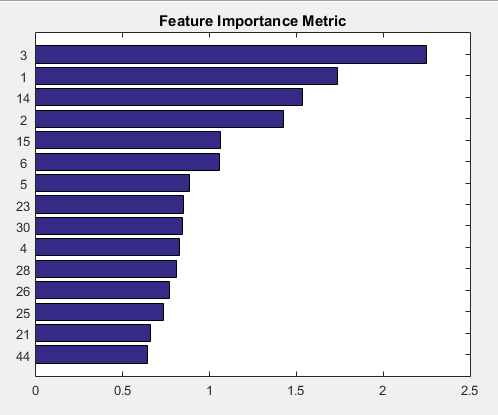
\includegraphics[scale=0.5]{FIM.png}}
		\end{center}
		\caption{Feature Importance Matrix Generated By Random Forest.}
		\label{fig:FIM}
	\end{figure}
	
		Table. \ref{table:Table1} provides us the evaluation parameters of all the models we have implemented. Plots \ref{fig:Plot1} and \ref{fig:Plot2} summarizes the data. 
		
		\begin{figure}[h]
			\begin{center}
				%\framebox[4.0in]{$\;$}
				\fbox{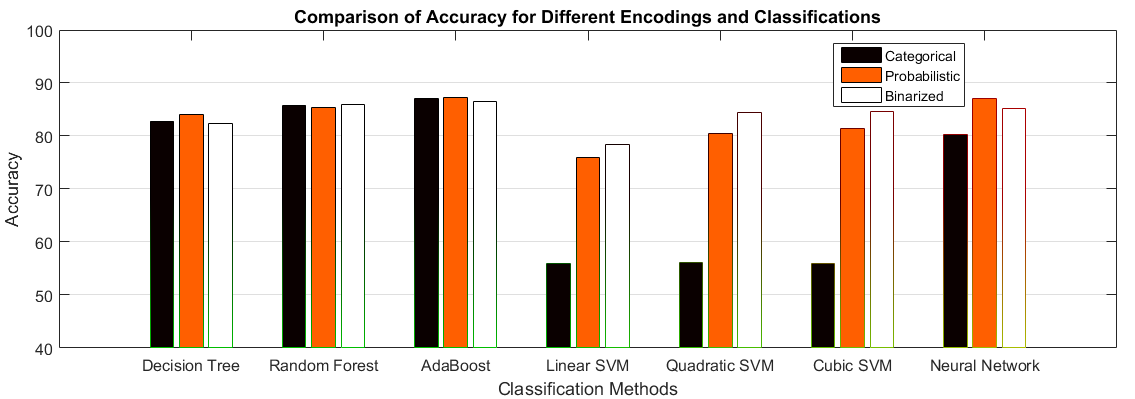
\includegraphics[scale=0.45]{Accuracy.png}}
			\end{center}
			\caption{Accuracy of the classification models implemented.}
			\label{fig:Plot1}
		\end{figure}
		
		\begin{figure}[h]
			\begin{center}
				%\framebox[4.0in]{$\;$}
				\fbox{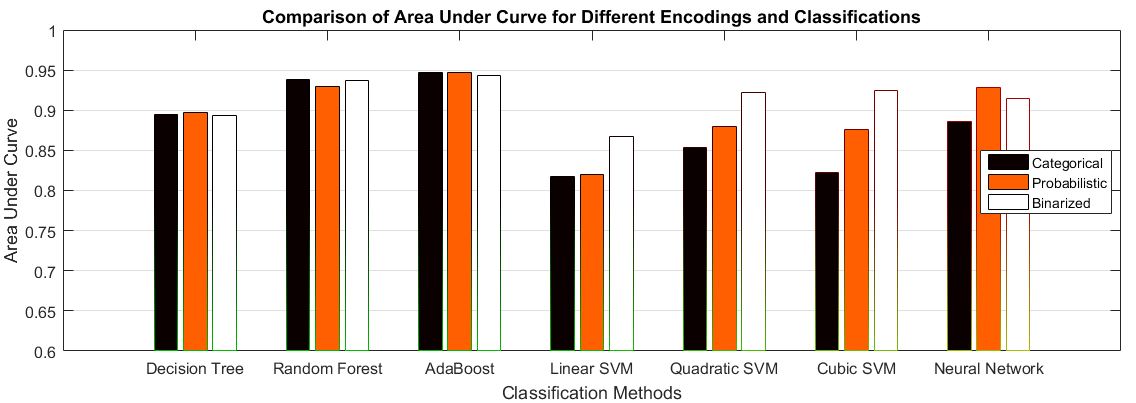
\includegraphics[scale=0.45]{AreaUnderCurve.png}}
			\end{center}
			\caption{Area Under Curve of the ROC curves for all the implemented classification models.}
			\label{fig:Plot2}
		\end{figure} 
		
		\renewcommand{\arraystretch}{1.5}
		\begin{table}[]
			\centering
			\resizebox{\textwidth}{!}{%
				\begin{tabular}{|l|l|l|l|l|l|}
					\hline
					\begin{tabular}[c]{@{}l@{}}Classification \\ Method\end{tabular} & \begin{tabular}[c]{@{}l@{}}Encoding \\ Method\end{tabular} & Accuracy (In \%) & Area Under Curve & TPR (In \%) & TNR(In \%) \\ \hline
					\multirow{3}{*}{Decision Tree}                                   & Categorical Data                                           & 82.8             & 0.895            & 86.26       & 79.68      \\ \cline{2-6} 
					& Binary Encoded                                             & 82.3             & 0.893            & 84.63       & 80.14      \\ \cline{2-6} 
					& Probability Encoded                                        & 84.0             & 0.897            & 82.54       & 85.29      \\ \hline
					\multirow{3}{*}{Random Forest}                                   & Categorical Data                                           & 85.8             & 0.938            & 86.05       & 85.58      \\ \cline{2-6} 
					& Binary Encoded                                             & 85.9             & 0.937            & 85.08       & 86.54      \\ \cline{2-6} 
					& Probability Encoded                                        & 85.4             & 0,930            & 82.6        & 87.9       \\ \hline
					\multirow{3}{*}{AdaBoost Tree}                                   & Categorical Data                                           & 87.1             & 0.947            & 87.35       & 86.82      \\ \cline{2-6} 
					& Binary Encoded                                             & 86.6             & 0.943            & 85.16       & 87.83      \\ \cline{2-6} 
					& Probability Encoded                                        & 87.3             & 0.947            & 86.52       & 87.85      \\ \hline
					\multirow{3}{*}{Linear SVM}                                      & Categorical Data                                           & 56.0             & 0.819            & 9.6         & 96.7       \\ \cline{2-6} 
					& Binary Encoded                                             & 78.4             & 0.867            & 73.67       & 82.62      \\ \cline{2-6} 
					& Probability Encoded                                        & 75.9             & 0.821            & 71.45       & 79.89      \\ \hline
					\multirow{3}{*}{Quadratic SVM}                                   & Categorical Data                                           & 56.1             & 0.839            & 9.5         & 97.1       \\ \cline{2-6} 
					& Binary Encoded                                             & 84.5             & 0.922            & 80.97       & 87.67      \\ \cline{2-6} 
					& Probability Encoded                                        & 80.5             & 0.880            & 75.94       & 84.52      \\ \hline
					\multirow{3}{*}{Cubic SVM}                                       & Categorical Data                                           & 55.9             & 0.806            & 9.1         & 97.1       \\ \cline{2-6} 
					& Binary Encoded                                             & 84.6             & 0.925            & 80.9        & 87.7       \\ \cline{2-6} 
					& Probability Encoded                                        & 80.8             & 0.875            & 77          & 84.2       \\ \hline
					\multirow{3}{*}{Neural Network}                                  & Categorical Data                                           & 80.3             & 0.886            & 78.0        & 81.3       \\ \cline{2-6} 
					& Binary Encoded                                             & 85.1             & 0.915            & 82.5        & 87.5       \\ \cline{2-6} 
					& Probability Encoded                                        & 87.1             & 0.928            & 85.14       & 88.84      \\ \hline
				\end{tabular}
			}
			\caption{Evaluation parameters obtained for all the tested classification models}
			\label{table:Table1}
		\end{table}
	
	
	\section{Conclusion}
	The experiments using the categorical values without encoding is done for decision tree, boosted trees and random forest, where we found boosted tree to be a little more accurate. Further, we will work on encoding the categorical attributes and create models based on neural networks, SVM and naive bayes classifiers.
	
	\begin{thebibliography}{10} % 100 is a random guess of the total number of
		%references
		\bibitem{Top10} Top 10 algorithms in data mining. Knowl. Inf. Syst. 14, 1 (December 2007), 1-37. DOI=http://dx.doi.org/10.1007/s10115-007-0114-2
		\bibitem{OneRow} Efficient “One-Row-per-Subject” Data Mart Construction for Data Mining, Gerhard Svolba, PhD, SAS Austria
		\bibitem{Multi} Reliable Early Classification on Multivariate Time Series with Numerical and Categorical Attributes, Cao, Tru et al.
		\bibitem{HighCard}Daniele Micci-Barreca. 2001. A preprocessing scheme for high-cardinality categorical attributes in classification and prediction problems. SIGKDD Explor. Newsl. 3, 1 (July 2001), 27-32. DOI=http://dx.doi.org/10.1145/507533.
		\bibitem{Matlab} Getting Started with Kaggle Data Science Competitions. Loren Shure
		\bibitem{Matlab} Predict Grant Applications - Kaggle Competition, https://www.kaggle.com/c/unimelb 
	\end{thebibliography}
	
	
\end{document}
